\chapter{算法实现与代表方案}

本章介绍已经接入通用协议的具体密码算法，并说明三组代表方案的选择依据。两种HIBE和五种常规
IBS形成十种端到端组合；Wang--PW是额外完成的目标参数矩阵SIS后端，目前与LATTE形成一套完整
组合。各算法保持独立参数和对象格式，公共协议仅通过第三章定义的接口调用。

\section{分层身份基加密实现}

\subsection{LATTE两层身份委派机制}

LATTE在NTRU结构中实现量子安全HIBE\cite{zhao2024latte}。作品采用LATTE-3参数：多项式次数
$N=1024$、模数$q=68718428161$、分层深度为2。主陷门由短NTRU关系构成，接收身份$r$和发送
身份$s$分别映射为两层身份多项式。发钥机构为$r$生成一级密钥，接收端再为$s$委派叶密钥。

加密端按$(r,s)$生成Ring-LWE型胶囊，叶密钥消去公开环项后恢复32字节随机种子。实现随后进行
确定性重加密核对，排除错误结果落入解码区间的情况。公开参数、主陷门、一级密钥、叶密钥和密文
采用不同对象类型，参数快照与对象一同保存。

实现复用LATTE作者代码中的Gaussian采样和ffSampling路径，并将原生对象封装为严格的Python
后端。每次原生采样后，适配层使用精确环算术检查NTRU关系、委派关系和对象形状。LATTE建立、
一级发钥和在线解密成本较低，因此A、B两组代表都选用该HIBE，使两组主要差别集中在IBS。

\subsection{Lai分层身份块扩展机制}

Lai方案利用理想格陷门完成分层委派\cite{lai2015trapdoors}。根公开向量与短陷门满足
\[
 \mathbf a_0^{\mathsf T}R+\mathbf a_1=\mathbf g.
\]
两层身份分别映射为二进制环元素$\mathrm{id}_1$和$\mathrm{id}_2$，完整身份公开项为
\[
 \mathbf a_{\mathrm{ID}}
 =\mathbf u_0+\mathrm{id}_1\mathbf u_1+\mathrm{id}_2\mathbf u_2.
\]
每委派一层，后端向公开矩阵追加身份块，并为扩展后的矩阵生成新陷门。接收身份对应第一层，认可
发送身份对应第二层。

C组采用$n=2048$、$q=274877976577$、$k=39$、深度2、$p=2$的C2配置。身份映射使用二进制
系数，避免身份乘短矩阵时放大噪声；叶陷门通过Babai反演恢复种子，并检查误差的模$p$结构。该
后端的主要成本是二级委派，因此第五章进一步引入接收会话，使固定身份对只生成一次叶密钥。

\section{身份基签名实现}

\subsection{BNN认证转换与ML-DSA／Falcon接入}

认证转换以普通数字签名为基础构造IBS\cite{galindo2006ibs}。系统建立时，发钥机构生成机构签名
密钥；为身份$s$发钥时，先生成用户普通签名密钥对$(\mathsf{vk}_s,\mathsf{xk}_s)$，再由机构
签署身份与用户验签公钥的规范编码：
\[
 \mathsf{cert}_s=\mathsf{DS.Sign}_{\mathsf{sk}_{\rm CA}}
       (\mathsf{Enc}(s,\mathsf{vk}_s)).
\]
完整IBS签名携带用户公钥、机构证书和用户签名。验证端先检查证书，再检查用户签名。

同一转换核心接入ML-DSA与Falcon。ML-DSA实现采用FIPS~204对象格式\cite{nist2024fips204}；
A组选用ML-DSA-44，其普通公钥为1,312字节、普通签名为2,420字节，转换后的IBS签名为6,237
字节。Falcon后端采用Falcon-512和Falcon-1024的固定作者实现及padded格式\cite{falcon2020}。
两者共享机构证书流程，但底层密钥、签名编码和版本号相互独立。

\subsection{Luo模格身份签名}

Luo后端实现原生模格IBS\cite{luo2024ibs}。身份哈希、消息挑战、响应和提示信息直接进入模格
签名关系，验证者使用公开参数、身份和消息完成验签。后端同时保留参考表示和无损紧凑表示，两种
格式加载后恢复为同一数学对象，签名与验签算法不变。

Luo分别与LATTE、Lai完成组合。它不属于A、B、C三组重点代表，但用于检验公共协议能否接入
另一类原生模格IBS，也为十种常规组合提供独立于SRGG的模格路线。

\subsection{SRGG身份目标与消息挑战关系}

SRGG采用模块格结构，公开矩阵写为
\[
 A=[I_d\mid\widehat A\mid B].
\]
身份$s$决定目标$h=H_1(P,s)$，用户短见证$y$满足$Ay=h\pmod Q$。签名构造矩阵和响应为
\[
 M_h=[\,2A\mid Qj-2h\,]\pmod{2Q},
 \qquad
 z=p_0+\begin{bmatrix}y\\1\end{bmatrix}(\zeta u+c),
\]
验证者由$W'=M_hz-Qjc$恢复承诺，重新计算挑战并检查响应范数\cite{jia2025ibs}。

B组采用PARAM-I：多项式次数$n=512$、模块秩2、$p=16383$、$Q=15744063$，参数评估中的
量子密钥恢复与伪造成本分别约为95 bit和93 bit。该后端包含大量不同取值范围的整数系数，参考
JSON对象较大。第五章的范围感知编码为公钥、主状态、用户密钥和签名分别选择位宽，在不改变
数学对象的前提下减少保存与传输字节。

\subsection{Sageloli环陷门与非齐次签名方程}

Sageloli的公开向量与主陷门$R$满足
\[
 A=[\bar A\mid g-\bar AR].
\]
为身份$s$发钥时，算法生成身份盐$\rho$并采样身份陷门$T_s$，使
\[
 AT_s=H_1(P,\rho,s)-g\pmod q.
\]
签名另取消息盐$\eta$，通过相关扰动和三进制陪集采样得到响应$z$；验证端检查范数和非齐次模
方程\cite{sageloli2023ibs}。

C组选用PARAM-I：$(d,k,\ell)=(2048,65,132)$、$q=3^{65}$、$r^2=49$。PARAM-II保持同一
算法并增大参数。论文参数下若把环乘法展开为普通矩阵，采样中间对象无法在常规工作站内保存。
第五章说明如何利用环结构和逐频率低秩计算完成两档参数的发钥与签名。

\subsection{Wang--PW目标参数矩阵SIS后端}

Wang--PW指Wang基本IBS与Pan--Wagner自适应转换组成的具体后端，它不是另一种“扩展IBS”
语法，也不同于第二章介绍的Wang通用IB-ME构造。该后端采用矩阵SIS关系，Pan--Wagner转换为
身份和消息分别加入随机盐\cite{wang2024ibme,pan2021ibs}。

目标参数为
\[
 n=512,\qquad q=4294967291,\qquad s_0=4.
\]
令$k=\lceil\log_2q\rceil=32$，gadget宽度$w=nk=16384$，公开矩阵宽度$m=32768$，签名向量
维数$M=49152$。根公开矩阵与陷门满足
\[
 A=[\bar A\mid G-\bar AR].
\]
身份密钥$X$满足$AX+H_1=G\pmod q$，签名短向量$z$满足
\[
 [A,H_1]z=H_2(P,\rho,s,\eta,M')\pmod q.
\]

有限离散Gaussian由独立原生组件执行，Python层负责域分隔哈希、参数快照、规范对象和精确模
方程。目标档采用约115 bit的量子安全工作值；公钥约64.0~MiB、主状态约576~MiB、用户签名
密钥约2.06~GiB、签名约384~KiB。
该实现已完成独立签验、状态恢复以及LATTE组合，实验章单列其服务器资源和分阶段时间。

\section{已实现算法与组合矩阵}

两种HIBE与五种常规IBS形成表~\ref{tab:implemented-matrix}所示的十种组合。每一格均通过统一
接口完成系统建立、双方发钥、消息加密、匹配解密和身份错配拒绝。同一算法的参数档或编码格式
不重复计为新方案。

\begin{table}[H]
\centering\small
\caption{两种HIBE与五种常规IBS的端到端组合}
\label{tab:implemented-matrix}
\begin{tabular}{@{}lccccc@{}}
\toprule
\rowcolor{black!8} HIBE & BNN＋ML-DSA & BNN＋Falcon & Luo & SRGG & Sageloli \\
\midrule
LATTE & 完成 & 完成 & 完成 & 完成 & 完成 \\
Lai & 完成 & 完成 & 完成 & 完成 & 完成 \\
\bottomrule
\end{tabular}
\end{table}

Wang--PW在常规十种组合之外单列。其目标参数对象远大于常规后端，目前完成LATTE＋Wang--PW
一套端到端组合。这样表述既保留“六种IBS均已接入”的实现事实，也不会把尚未运行的Lai＋
Wang--PW计入组合矩阵。

\section{代表方案的性能指标与选取依据}

十种常规组合用于验证通用性，A、B、C三组用于深入说明不同成本分布。A与B固定LATTE，便于
观察认证转换和原生模格IBS的差别；C同时采用Lai与Sageloli，用于研究高成本委派、环格采样和
会话复用。表~\ref{tab:representatives}先列出算法和容量。

\begin{table}[H]
\centering\small
\caption{三组代表的算法构成与应用消息容量}
\label{tab:representatives}
\begin{tabularx}{\textwidth}{@{}cp{.16\textwidth}Xp{.18\textwidth}@{}}
\toprule
\rowcolor{black!8} 组 & HIBE & IBS & 应用消息上限 \\
\midrule
A & LATTE-3 & BNN／ML-DSA-44 & 59,191 B \\
B & LATTE-3 & SRGG PARAM-I紧凑格式 & 65,364 B \\
C & Lai C2 & Sageloli PARAM-I & 3,924 B \\
\bottomrule
\end{tabularx}
\end{table}

表~\ref{tab:representative-indicators}汇总当前可直接用于理解使用方式的原始指标。A、B数据来自
同机重复实验；C的完整运行和接收会话来自另一台机器，因此该表保留测量条件，不把三组折算为
单一总分。

\begin{table}[H]
\centering\small
\caption{三组代表的主要性能与资源指标}
\label{tab:representative-indicators}
\begin{tabularx}{\textwidth}{@{}>{\raggedright\arraybackslash}p{.27\textwidth}>{\raggedright\arraybackslash}X>{\raggedright\arraybackslash}X>{\raggedright\arraybackslash}X@{}}
\toprule
\rowcolor{black!8} 指标 & A & B & C \\
\midrule
重复／在线加密 & 0.0785 s（中位数） & 9.17 s（中位数） & 99.0 s（单次完整运行） \\
重复／会话后解密 & 0.152 s（中位数） & 0.161 s（中位数） & 28.6 s（会话后中位数） \\
首次完整解密 & 0.284 s & 0.239 s & 425 s，其中委派393 s \\
完整密文 & 约139 KiB & 约146 KiB & 约4.34 MiB \\
主要资源位置 & 发送与接收均为低延迟 & 发送端SRGG签名 & 接收端Lai委派、较大密文 \\
\bottomrule
\end{tabularx}
\end{table}

图~\ref{fig:representative-profile}参考多指标性能图的表达方式，将在线加密时间、在线接收时间、
完整密文长度和应用容量映射为0--100的“使用特征分值”。耗时和长度采用“越小越高”，容量采用
“越大越高”；映射在对数尺度上按本图三组的最好值归一化。原始数值仍以表
~\ref{tab:representative-indicators}和表~\ref{tab:representatives}为准，雷达图用于观察组合特征，
不代替同机性能表。

\begin{figure}[H]
\centering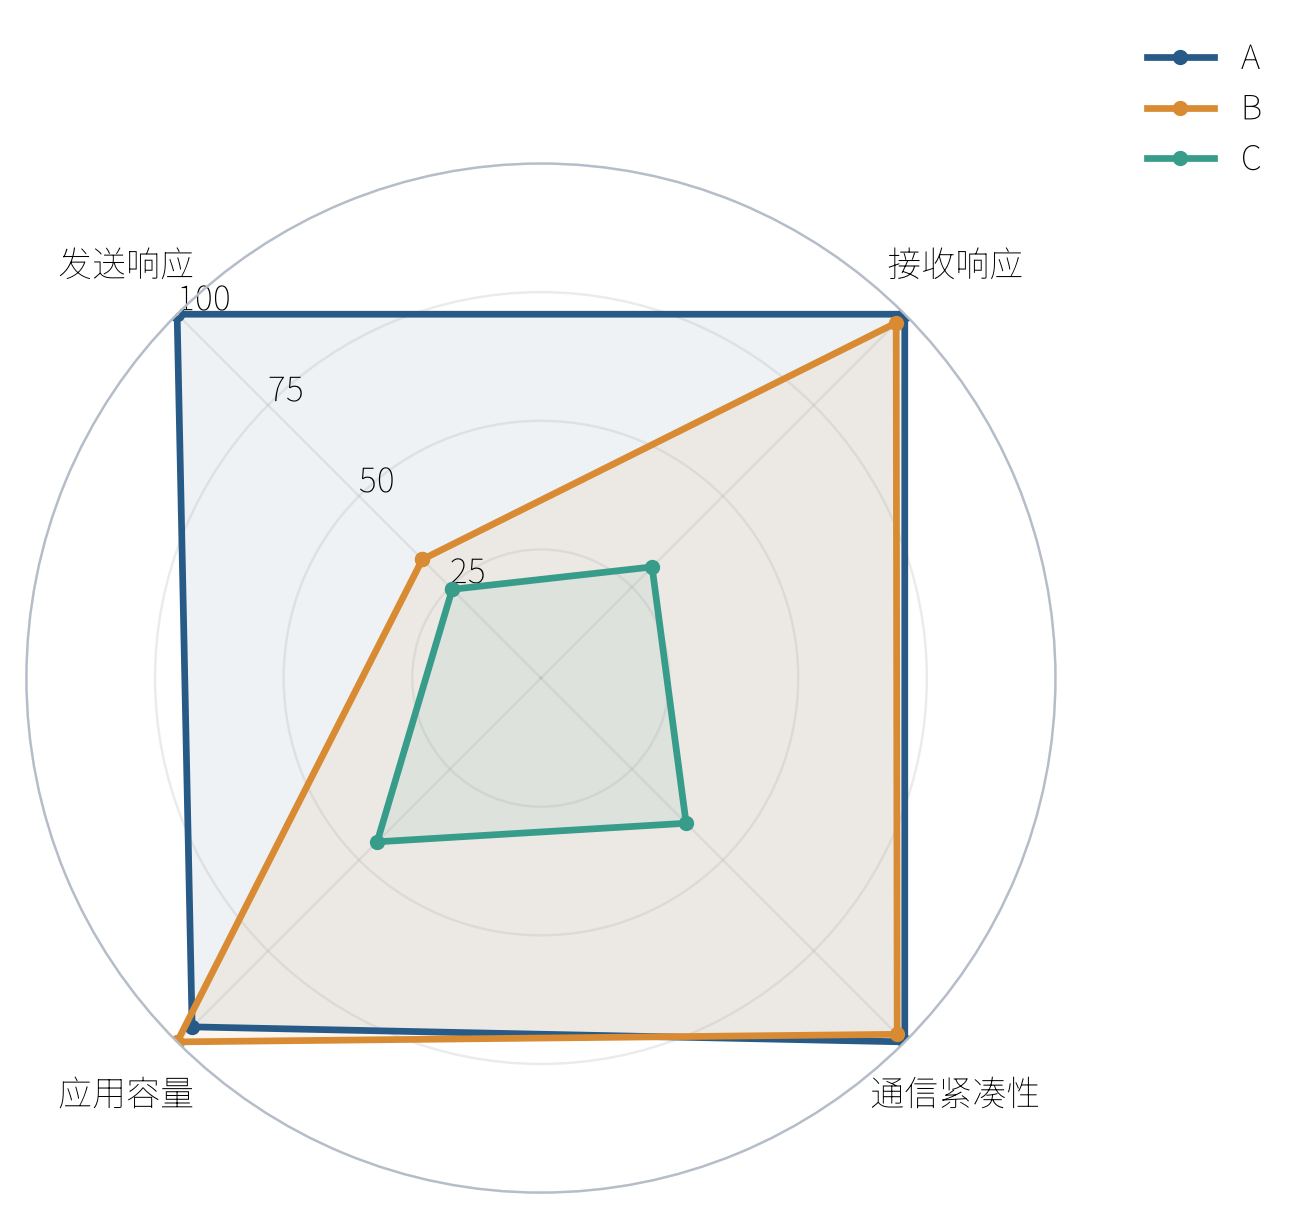
\includegraphics[width=.78\textwidth]{figures/representative-profile.png}
\caption{三组代表的归一化使用特征；分值越高表示对应指标越有利}
\label{fig:representative-profile}
\end{figure}

\section{三组代表的应用定位}

\subsection{A组：低延迟定向消息}

A组采用LATTE-3与BNN／ML-DSA-44。其重复加密和解密均处于亚秒级，适合需要交互响应的机构
消息、浏览器演示和频繁的小消息收发。ML-DSA组件具有固定标准对象格式，认证转换也便于复用
普通签名实现。A组的主要通信开销来自一次性认证而不是IBS签名，因此后续优化重点是外层认证
结构和整包长度。

\subsection{B组：原生模格身份认证与紧凑状态}

B组采用LATTE-3与SRGG PARAM-I。其接收端时间与A接近，主要额外成本集中在发送者发钥和
签名。范围感知编码显著减少SRGG主状态、用户密钥和签名长度。该组适合发送端能够承担数秒签名、
接收端需要快速验证的批量定向投递，也适合研究原生模格IBS和紧凑对象在完整协议中的作用。

\subsection{C组：固定身份对的连续通信}

C组采用Lai C2与Sageloli PARAM-I。初次解密需要完成高成本叶钥委派，密文也明显大于A、B；
建立接收会话后，同一身份对的后续解密不再重复委派。因而，C组更适合双方身份固定、允许离线
准备并连续处理多条消息的使用方式，例如固定管理端与受控终端之间的周期消息。其价值在于展示
高成本HIBE与环格IBS如何通过结构化采样和会话复用进入完整系统，而不是作为低延迟基线。

\section{本章小结}

本章说明了两种HIBE与六种IBS的算法关系和实现对象，并区分十种常规组合与LATTE＋Wang--PW
目标参数组合。A、B、C三组分别代表低延迟认证转换、原生模格身份签名和固定身份对的高成本
环格路线。下一章集中展开Sageloli采样、SRGG编码和Lai会话三项关键优化。
